\chapter{Approach}
The first section Research protocol \ref{section-research-protocol} describes the how the investigation of the problem formulation has been performed. The following section, Measuring Lines of Code \ref{section-measuring-lines-of-code}, states how the software metric logical lines of code has been used as a measurement of the result. The last section, Layer communication \ref{section-layer-communication}, explains how the relationship between the mobile and web application layer were evaluated. 


\section{Research protocol} \label{section-research-protocol}
To carry out the investigation proposed in the problem formulation a practical approach has been used. To evaluate and compare the two different methods a mobile application described in \ref{subsection-mobile-application} with the same requirements were developed in each method. The mobile application needs an existing web application and therefore a simple web application described in \ref{subsection-web-application} were developed first of all. The web application were developed in the framework Ruby on Rails. 

We have used ourself as the developers of the web application and as the developers of the mobile application in both methods. The experiences and thoughts when developing were logged in a journal. After the mobile applications were developed the architecture were visualized in a UML diagram and the different classes were described. The UML diagram shows the methods of the classes but hides the attributes of the classes for the sake of better clarity. 

\subsection{The web application} \label{subsection-web-application}
The used web application comprises of a single page and is compatible with the web browser Google Chrome. The page displays a form with a text field, a take photo button, an upload photo button, a location button and a submit button, see figure \ref{fig:nativeuml}. When the upload photo or take photo or location button is pressed the web application uses the Google Chrome’s built in ability to take a photo or upload a photo or get the location.

\begin{figure}[h!]
	\centering
    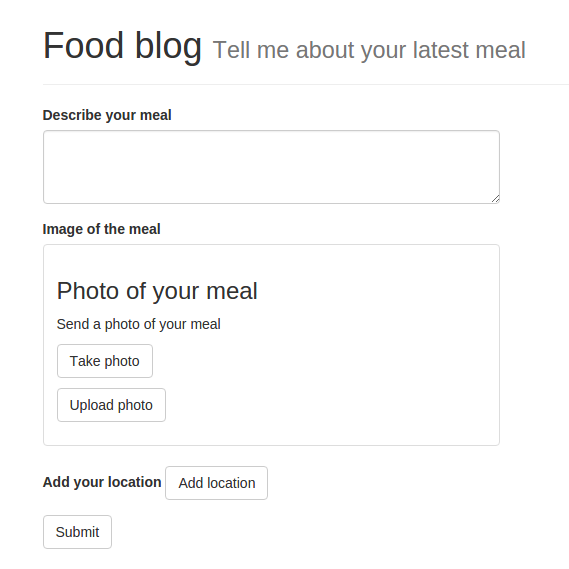
\includegraphics[width=120mm,natwidth=800,natheight=600]{./img/webAppFrontPage.png}
    \caption{The web app front page displayed in a browser}
    \label{fig:nativeuml}
\end{figure}

\subsection{The mobile application} \label{subsection-mobile-application}
The mobile applications consist of two parts. The web application described above and the mobile application encapsulating the web application. The mobile application must encapsulate the web application and display the web application exactly the same way as it is displayed in a browser. The mobile application must use the mobile’s native functions to get the value for the image and the location. The mobile application has no knowledge of the back-end of the web application. It merely communicates with the client-side of the web application.

The text field in the web application has no connection to the mobile application layer. 

For taking or uploading the image value in the form the mobile application must an existing image from the image gallery or take a picture using the camera on the phone. The photo passed back to the web application must be in Base64 format. 

The location must be obtained using the mobile’s GPS. 

When the user interacts with the mobile application the interaction must be directly with the web application encapsulated within the mobile application. 

In the project the following was used for developing and testing:
\begin{itemize}
\item Version 21 of the Android SDK when developing using the Android application framework.
\item Apache Cordova CLI version 4.0 when developing using the PhoneGap framework. 
The mobile that was used when testing the mobile applications was a Nexus 5 mobile with the Android version 5.1.1.
\item The web application has been tested in the Google Chrome browser version 44.0.2403.157.
\end{itemize}

\section{Measuring lines of code}\label{section-measuring-lines-of-code}
The resulting mobile applications are measured using a software metric namely logical lines of code. To count logical lines of code Project Code Meter has been used which ignores the following lines of code \cite{project-code-meter2015}

\begin{itemize}
\item Auto-generated code lines.
\item Header files.
\item Ineffective code statements.
\item Pragma compiler directives.
\item Labels.
\item Switch cases are not statements by themselves (so empty "case").
\item Several statements on the same physical line are counted as several LLOC.
\end{itemize}

The mobile application were written in two different programming languages, Java and JavaScript. To compare the measurement result of logical lines of code we use the conversion table described by Galorath and Evans \cite[p.~163]{galorath2006}. JavaScript and Java are both third generation languages and therefore the conversion is roughly 1 to 1. 

The logical lines of code written in the web application layer is also measured in both developing methods. To give an correct result we measured the added logical lines of code that have been written as a result of the mobile application. The resulting lines in the mobile and web application layer is added together to give a total result. 

The logical lines of code in the web application layer is also measured in both developing methods. The resulting lines in the mobile and web application layer is added together to give a total result. 

\section{Layer communication} \label{section-layer-communication}
A prerequisite is that the communication between the mobile application and web application layer has a master and slave relationship. To evaluate this communication a flow diagram of the web layer sending a request for native data and the mobile application layer responding with data is constructed. The flow diagram acts as a suggestion in how developer friendly the communication is combined with our personal developing experiences.